\documentclass[aspectratio=169,11pt,t]{beamer}

% ============================================================
% Theme and typography
% ============================================================
\usetheme{Madrid}
\usecolortheme{default}
\usefonttheme{professionalfonts}
\setbeamertemplate{navigation symbols}{}
\setbeamertemplate{headline}{}

\setbeamertemplate{footline}{%
  \leavevmode\hbox{%
  \begin{beamercolorbox}[wd=.82\paperwidth,ht=2.5ex,dp=1.0ex,leftskip=.8em]{author in head/foot}
    CSCI 2406 --- Computer Organization \& Architecture
  \end{beamercolorbox}%
  \begin{beamercolorbox}[wd=.18\paperwidth,ht=2.5ex,dp=1.0ex,rightskip=.8em]{date in head/foot}
    \hfill\insertframenumber/\inserttotalframenumber
  \end{beamercolorbox}}
}

\setbeamersize{text margin left=0.7cm,text margin right=0.7cm}
\setbeamerfont{frametitle}{size=\Large,series=\bfseries}
\setbeamerfont{block title}{size=\normalsize,series=\bfseries}
\setbeamertemplate{blocks}[rounded][shadow=false]
\addtobeamertemplate{block begin}{\vspace{0.05em}}{\vspace{0.05em}}
\addtobeamertemplate{block end}{}{\vspace{0.10em}}
\setbeamertemplate{itemize/enumerate body begin}{\setlength{\itemsep}{3pt}}
\setbeamertemplate{itemize/enumerate subbody begin}{\setlength{\itemsep}{2pt}}

% ============================================================
% Packages
% ============================================================
\usepackage[T1]{fontenc}
\usepackage{lmodern}
\usepackage[scale=0.92]{sourcecodepro}
\usepackage{amsmath}
\usepackage{booktabs}
\usepackage{array}
\usepackage{colortbl}
\usepackage{tikz}
\usetikzlibrary{arrows.meta,positioning,calc}

% ============================================================
% Colors
% ============================================================
\definecolor{navy}{RGB}{24,43,68}
\definecolor{deepblue}{RGB}{45,88,130}
\definecolor{softgray}{RGB}{245,247,250}
\definecolor{darkgray}{RGB}{25,28,32}
\definecolor{gold}{RGB}{200,145,35}

\setbeamercolor{palette primary}{bg=navy,fg=white}
\setbeamercolor{palette secondary}{bg=deepblue,fg=white}
\setbeamercolor{frametitle}{bg=navy,fg=white}
\setbeamercolor{title}{fg=white}
\setbeamercolor{subtitle}{fg=white}
\setbeamercolor{author}{fg=white}
\setbeamercolor{date}{fg=white}
\setbeamercolor{titlelike}{fg=white}
\setbeamercolor{block title}{bg=deepblue,fg=white}
\setbeamercolor{block body}{bg=softgray,fg=darkgray}
\setbeamercolor{normal text}{fg=darkgray,bg=white}

% ============================================================
% Formatting shortcuts
% ============================================================
\setlength{\parskip}{0pt}

\newcommand{\key}[1]{\textbf{#1}}
\newcommand{\bits}[1]{\texttt{#1}}
\newcommand{\hex}[1]{\texttt{0x#1}}
\newcommand{\code}[1]{\texttt{#1}}

% ============================================================
% Section divider
% ============================================================
\newcommand{\sectiondivider}[2]{%
\begin{frame}[plain]

\begin{tikzpicture}[remember picture,overlay]
\fill[navy] (current page.south west) rectangle (current page.north east);
\fill[gold] (current page.south west)
  rectangle ([yshift=.15cm]current page.south east);
\end{tikzpicture}

\vspace*{\fill}

\begin{minipage}{0.94\textwidth}
\raggedright
\hyphenpenalty=10000
\exhyphenpenalty=10000

{\color{gold}\large\bfseries #1\par}

\vspace{0.3cm}

{\color{white}\fontsize{22}{26}\selectfont\bfseries
#2\par}

\end{minipage}

\vspace*{\fill}

\end{frame}
}

% ============================================================
% Metadata
% ============================================================
\title[Topic 4]{Integer Arithmetic and Performance Basics}
\subtitle{Fixed-width arithmetic, condition flags, shifts, and CPU execution-time analysis}
\author{Computer Organization \& Architecture}
\date{Topic 4}

\begin{document}










% ============================================================
% Slide 1
% ============================================================

\begin{frame}[plain]
\begin{tikzpicture}[remember picture,overlay]
\fill[navy] (current page.south west) rectangle (current page.north east);
\fill[gold] (current page.south west) rectangle ([yshift=.15cm]current page.south east);
\end{tikzpicture}

\vspace*{\fill}

\begin{minipage}{0.88\textwidth}
{\color{gold}\normalsize\bfseries
CSCI 2406 \;|\; Computer Organization \& Architecture \;|\; TOPIC 4
\par}

\vspace{0.25cm}

{\color{white}\fontsize{24}{28}\selectfont\bfseries
Integer Arithmetic and\\[0.08cm]Performance Basics
\par}

\vspace{0.35cm}

{\color{white!80}\large
Integer arithmetic, condition flags,\\clock rate, CPI, and execution time
\par}
\end{minipage}

\vfill

{\color{white!70}\small
Dr. J. Burns
\par}

\vspace*{\fill}
\end{frame}










% ============================================================
% Slide 2
% ============================================================

\begin{frame}{Topic 4 Outline}
\begin{block}{Topic Objective}
Understand how fixed-width integer arithmetic works at the machine level, how condition flags support later control flow, and how instruction count, CPI, and clock rate determine execution time.
\end{block}
\vspace{0.25cm}
\begin{itemize}
\item \key{Section 1}: Fixed-width addition, subtraction, and interpretation
\item \key{Section 2}: Condition flags and AArch64 comparison behavior
\item \key{Section 3}: Multiplication, division, and shifts
\item \key{Section 4}: Clock rate, CPI, and execution time
\item \key{Section 5}: Summary and self-test
\end{itemize}
\end{frame}

\sectiondivider{Section 1}{Fixed-Width Integer Arithmetic}










% ============================================================
% Slide 3
% ============================================================

\begin{frame}{Integer Arithmetic}
\begin{block}{Integer Operations Are Everywhere}
Integer arithmetic is not limited to explicit calculator-like expressions. It appears constantly in address calculation, loop control, array indexing, comparisons, and resource accounting.
\end{block}
\vspace{0.25cm}
\begin{columns}[T,onlytextwidth]
\column{0.48\textwidth}
\begin{block}{Program-Level Examples}
\begin{itemize}
\item Increment loop counters.
\item Compute array offsets.
\item Compare bounds and indices.
\item Update pointer values.
\end{itemize}
\end{block}
\column{0.48\textwidth}
\begin{block}{Hardware-Level Consequence}
\begin{itemize}
\item Arithmetic uses fixed-width registers.
\item Only the destination-width result bits are retained.
\item Flags record selected facts about results.
\item Interpretation is supplied by software.
\end{itemize}
\end{block}
\end{columns}
\end{frame}



% ============================================================
% Slide 4
% ============================================================

\begin{frame}{Arithmetic Operates on Bit Patterns}

\begin{columns}[T,onlytextwidth]

\column{0.48\textwidth}
\begin{block}{Hardware View}
\begin{itemize}
  \item The ALU operates on fixed-width bit patterns.
  \item It does not know whether the programmer intends signed or unsigned meaning.
  \item The register width determines how many result bits are kept.
\end{itemize}
\end{block}

\column{0.48\textwidth}
\begin{block}{Programmer View}
\begin{itemize}
  \item \key{Unsigned:} interpret the bits as a non-negative integer.
  \item \key{Signed:} interpret the bits using two's complement.
  \item \key{Flags:} record selected facts about the fixed-width result.
\end{itemize}
\end{block}

\end{columns}

\vspace{0.2cm}

\begin{block}{Connection to Topic 3}
Topic 3 covered numeric ranges and two's-complement representation. Here the focus is arithmetic results and condition flags.
\end{block}

\end{frame}









% ============================================================
% Slide 5
% ============================================================

\begin{frame}{Binary Addition and Carry}


\vspace{-0.35cm}
\begin{columns}[T,onlytextwidth]

\column{0.48\textwidth}
\begin{block}{Column Addition}
Binary addition proceeds bit by bit. A carry-out from one column becomes the carry-in to the next column.

\vspace{0.08cm}

\begin{center}
\setlength{\tabcolsep}{0.28em}
\renewcommand{\arraystretch}{1.05}
\begin{tabular}{rccccc}
\multicolumn{1}{r}{} & \scriptsize carry: & \scriptsize 1 & \scriptsize 1 & \scriptsize 1 & \scriptsize 1 \\
\multicolumn{1}{r}{} &              & 1 & 1 & 1 & 1 \\
\multicolumn{1}{r}{$+$} &            & 0 & 0 & 0 & 1 \\
\cline{3-6}
\multicolumn{1}{r}{} & \scriptsize result: & 0 & 0 & 0 & 0 \\
\multicolumn{1}{r}{} & \scriptsize carry-out: & \multicolumn{4}{c}{1}
\end{tabular}
\end{center}

\end{block}

\column{0.48\textwidth}
\begin{block}{Unsigned Meaning}
\begin{itemize}
\item In 4 bits, only the lower \code{0000} remains.
\item The extra bit is the carry-out.
\item For unsigned arithmetic, carry-out means the mathematical result exceeded the available range.
\end{itemize}
\end{block}

\end{columns}

\vspace{0.05cm}

\begin{block}{Fixed-Width Result}\small
An $n$-bit register keeps only $n$ result bits. Extra information may be reflected in condition flags.
\end{block}

\end{frame}





% ============================================================
% Slide 6
% ============================================================

\begin{frame}{Subtraction and Condition Flags}

\begin{block}{Representation}
Topic 3 showed how two's-complement values are represented and how subtraction can be performed by adding a negated operand.
\end{block}

\vspace{0.25cm}

\begin{block}{Focus in This Topic}
Here the focus is not the representation method itself. The focus is what arithmetic does to a fixed-width result and which condition flags are set.
\end{block}

\vspace{0.25cm}

\begin{itemize}\setlength{\itemsep}{6pt}
  \item The register keeps the fixed-width result bits.
  \item NZCV records selected facts about that result.
  \item Signed and unsigned interpretations use different flags.
\end{itemize}

\end{frame}














% ============================================================
% Slide 7
% ============================================================

\begin{frame}{Signed vs. Unsigned Interpretation}
\begin{block}{Same Bits, Different Values}
The same bit pattern can have different numeric meanings depending on whether software treats it as unsigned or signed two's complement.
\end{block}
\vspace{0.15cm}
\begin{center}
\small
\renewcommand{\arraystretch}{1.15}
\begin{tabular}{
>{\raggedright\arraybackslash}m{3.0cm}
>{\raggedright\arraybackslash}m{3.0cm}
>{\raggedright\arraybackslash}m{4.3cm}
}
\rowcolor{navy}
{\color{white}\bfseries 8-bit pattern} &
{\color{white}\bfseries Unsigned} &
{\color{white}\bfseries Signed two's complement} \\
\rowcolor{softgray}
\code{01111111} & 127 & 127 \\
\rowcolor{white}
\code{10000000} & 128 & $-128$ \\
\rowcolor{softgray}
\code{11111111} & 255 & $-1$ \\
\end{tabular}
\end{center}
\vspace{0.2cm}
\begin{block}{Connection to AArch64}
The instruction result is a bit pattern. The choice of signed or unsigned branch determines how flags are interpreted later.
\end{block}
\end{frame}

\sectiondivider{Section 2}{Condition Flags and Comparisons}










% ============================================================
% Slide 8
% ============================================================

\begin{frame}{Why Condition Flags?}
\begin{block}{Arithmetic Produces More Than a Result}
A fixed-width arithmetic operation produces a register result, but later instructions may also need to know whether that result was zero, negative, produced a carry-out, or caused signed overflow.
\end{block}
\vspace{0.2cm}
\begin{itemize}
\item These properties are recorded in four condition flags: \code{N}, \code{Z}, \code{C}, and \code{V}.
\item Flag-setting arithmetic updates NZCV while also computing the normal register result.
\item Comparison instructions update NZCV without keeping the arithmetic result.
\item Conditional branches then test these flags to make control-flow decisions.
\end{itemize}
\vspace{0.15cm}
\begin{block}{Why This Matters}
NZCV connects arithmetic to decisions such as equality, signed ordering, and unsigned ordering.
\end{block}
\end{frame}










% ============================================================
% Slide 9
% ============================================================

\begin{frame}{NZCV Condition Flags}
\vspace{-0.25cm}
\begin{block}{Processor Status}
AArch64 maintains architectural processor state in \key{PSTATE}. Four condition-code bits within that state record selected properties of arithmetic and logical results and are collectively called \key{NZCV}.
\end{block}
\begin{center}
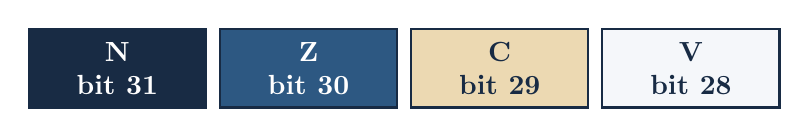
\begin{tikzpicture}[
  fld/.style={
    draw=navy,
    thick,
    minimum width=2.25cm,
    minimum height=1.0cm,
    align=center,
    font=\bfseries
  }
]
\node[fld,fill=navy,text=white] (n) {N\\bit 31};
\node[fld,fill=deepblue,text=white,right=.15cm of n] (z) {Z\\bit 30};
\node[fld,fill=gold!35,text=navy,right=.15cm of z] (c) {C\\bit 29};
\node[fld,fill=softgray,text=navy,right=.15cm of c] (v) {V\\bit 28};
\end{tikzpicture}
\end{center}
\vspace{-0.15cm}
\begin{itemize}
\item \key{N}: most-significant bit of the result is 1.
\item \key{Z}: result is exactly zero.
\item \key{C}: records carry-out for addition and supports unsigned comparison after subtraction.
\item \key{V}: indicates signed two's-complement overflow.
\end{itemize}
\vspace{0.05cm}
\begin{block}{NZCV Representation}
When NZCV is accessed as a system-register value, the four flags occupy bits 31--28 in the order \code{N Z C V}.
\end{block}
\end{frame}










% ============================================================
% Slide 10
% ============================================================

\begin{frame}{Flag-Setting Arithmetic}
\begin{columns}[T,onlytextwidth]
\column{0.48\textwidth}
\begin{block}{No Flag Update}
\large
\hspace{1.4cm}\code{add x0, x1, x2}\\[0.12cm]
\hspace{1.4cm}\code{sub x0, x1, x2}
\normalsize
\begin{itemize}
\item Write a register result.
\item Leave NZCV unchanged.
\end{itemize}
\end{block}
\column{0.48\textwidth}
\begin{block}{Flag Update}
\large
\hspace{1.4cm}\code{adds x0, x1, x2}\\[0.12cm]
\hspace{1.4cm}\code{subs x0, x1, x2}
\normalsize
\begin{itemize}
\item Write a register result.
\item Update NZCV from that operation.
\end{itemize}
\end{block}
\end{columns}
\vspace{0.25cm}
\begin{block}{AArch64 Detail}
Flag updates are provided by specific instruction forms such as \code{adds} and \code{subs}; this is not a general rule of simply adding an \code{s} to every mnemonic.
\end{block}
\end{frame}










% ============================================================
% Slide 11
% ============================================================

\begin{frame}{N: Negative Flag}
\vspace{-0.2cm}
\begin{block}{When N Is Set}
For a flag-setting arithmetic operation, \code{N=1} when the most-significant bit of the destination-width result is 1.
\end{block}
\begin{columns}[T,onlytextwidth]
\column{0.48\textwidth}
\begin{block}{Example}
\large
\hspace{1.2cm}\code{3 - 5 = 1110}
\normalsize
\begin{itemize}
\item In 4-bit two's complement, \code{1110} represents $-2$.
\item The sign bit is 1, so \code{N=1}.
\end{itemize}
\end{block}
\column{0.48\textwidth}
\begin{block}{AArch64 Context}
\large
\hspace{1.1cm}\code{subs x0, x1, x2}
\normalsize
\begin{itemize}
\item Writes the subtraction result to \code{x0}.
\item Updates NZCV from that result.
\item Ordinary \code{sub} leaves NZCV unchanged.
\end{itemize}
\end{block}
\end{columns}
\vspace{-0.05cm}
\begin{block}{Important Limitation}
Signed less-than uses \code{N} together with \code{V}; \code{N} alone is not sufficient.
\end{block}
\end{frame}










% ============================================================
% Slide 12
% ============================================================

\begin{frame}{Z: Zero Flag}
\begin{block}{When Z Is Set}
\code{Z=1} when every bit of the destination-width result is zero.
\end{block}
\vspace{0.2cm}
\begin{columns}[T,onlytextwidth]
\column{0.48\textwidth}
\begin{block}{Arithmetic Example}
\large
\hspace{1.3cm}\code{0101 - 0101 = 0000}
\normalsize
\begin{itemize}
\item The result is exactly zero.
\item Therefore \code{Z=1}.
\end{itemize}
\end{block}
\column{0.48\textwidth}
\begin{block}{Comparison Example}
\large
\hspace{1.5cm}\code{cmp x0, x1}
\normalsize
\begin{itemize}
\item \code{cmp} evaluates \code{x0 - x1} for flags.
\item If \code{x0 == x1}, the difference is zero.
\item Therefore \code{Z=1}.
\end{itemize}
\end{block}
\end{columns}
\vspace{0.15cm}
\begin{block}{Branch Connection}
After a comparison, \code{b.eq} tests \code{Z=1}; \code{b.ne} tests \code{Z=0}.
\end{block}
\end{frame}










% ============================================================
% Slide 13
% ============================================================

\begin{frame}{C: Carry Flag}
\begin{block}{Addition}
For addition, \code{C=1} when the fixed-width addition produces a carry out of the most-significant bit. Only the low $n$ result bits are stored in an $n$-bit destination.
\end{block}
\vspace{0.12cm}
\begin{columns}[T,onlytextwidth]
\column{0.46\textwidth}
\begin{block}{4-Bit Addition}
\large
\hspace{1.2cm}\code{1111 + 0001}\\[0.08cm]
\hspace{1.2cm}\code{= 1 0000}
\normalsize
\begin{itemize}
\item Stored result: \code{0000}.
\item Carry out: 1.
\item Therefore \code{C=1}.
\end{itemize}
\end{block}
\column{0.50\textwidth}
\begin{block}{Subtraction Uses the Same Adder}
\[
A-B=A+(\sim B)+1
\]
\small
\hspace{0.15cm}\code{5 - 3: 0101 + 1101 = 1 0010}\\[0.08cm]
\hspace{0.15cm}\code{3 - 5: 0011 + 1011 = 1110}
\normalsize
\begin{itemize}
\item Carry out $\Rightarrow$ \code{C=1} and $5\ge3$.
\item No carry out $\Rightarrow$ \code{C=0} and $3<5$.
\end{itemize}
\end{block}
\end{columns}
\end{frame}










% ============================================================
% Slide 14
% ============================================================

\begin{frame}{C After Subtraction}
\begin{block}{Unsigned Interpretation}
For the subtraction $A-B$, the carry flag provides information about the unsigned relationship between the two operands.
\end{block}
\vspace{0.18cm}
\begin{center}
\small
\renewcommand{\arraystretch}{1.18}
\begin{tabular}{
>{\raggedright\arraybackslash}m{2.4cm}
>{\raggedright\arraybackslash}m{3.2cm}
>{\raggedright\arraybackslash}m{4.8cm}
}
\rowcolor{navy}
{\color{white}\bfseries Condition} &
{\color{white}\bfseries Carry flag} &
{\color{white}\bfseries Unsigned interpretation} \\
\rowcolor{softgray}
$A\ge B$ &
\code{C=1} &
The fixed-width subtraction produces a carry out. \\
\rowcolor{white}
$A<B$ &
\code{C=0} &
The fixed-width subtraction does not produce a carry out. \\
\end{tabular}
\end{center}
\vspace{0.2cm}
\begin{block}{AArch64 Comparison Use}
After \code{cmp x0, x1}, \code{C=1} corresponds to \code{x0 >= x1} for unsigned values, while \code{C=0} corresponds to \code{x0 < x1}.
\end{block}
\end{frame}










% ============================================================
% Slide 15
% ============================================================

\begin{frame}{V: Signed Overflow Flag}
\begin{block}{Signed Addition Rule}
For signed addition, overflow occurs when two operands with the same sign produce a result with the opposite sign.
\end{block}
\vspace{0.12cm}
\begin{columns}[T,onlytextwidth]
\column{0.48\textwidth}
\begin{block}{Positive + Positive}
\large
\hspace{1.0cm}\code{0111 + 0001 = 1000}
\normalsize
\begin{itemize}
\item $7+1=8$ cannot be represented in 4-bit signed arithmetic.
\item Two positive operands produced a negative result pattern.
\item Therefore \code{V=1}.
\end{itemize}
\end{block}
\column{0.48\textwidth}
\begin{block}{Negative + Negative}
\large
\hspace{1.0cm}\code{1000 + 1111 = 0111}
\normalsize
\begin{itemize}
\item $-8+(-1)=-9$ cannot be represented in 4 bits.
\item Two negative operands produced a positive result pattern.
\item Therefore \code{V=1}.
\end{itemize}
\end{block}
\end{columns}
\vspace{-0.03cm}
\small
Adding operands with opposite signs does not produce signed overflow in addition.
\normalsize
\end{frame}










% ============================================================
% Slide 16
% ============================================================

\begin{frame}{Signed Overflow in Subtraction}
\begin{block}{Subtraction Rule}
For signed subtraction \code{A - B}, overflow can occur only when \code{A} and \code{B} have opposite signs and the result sign differs from the sign of \code{A}.
\end{block}
\vspace{0.18cm}
\begin{columns}[T,onlytextwidth]
\column{0.48\textwidth}
\begin{block}{Positive Minus Negative}
A positive value minus a negative value should become more positive. If the fixed-width result becomes negative, signed overflow occurred.
\end{block}
\column{0.48\textwidth}
\begin{block}{Negative Minus Positive}
A negative value minus a positive value should become more negative. If the fixed-width result becomes positive, signed overflow occurred.
\end{block}
\end{columns}
\vspace{0.2cm}
\begin{block}{Different Roles}
\code{C} supports unsigned reasoning after subtraction; \code{V} records whether the signed subtraction exceeded the representable signed range.
\end{block}
\end{frame}










% ============================================================
% Slide 17
% ============================================================

\begin{frame}{Comparison with \code{cmp}}
\begin{block}{\code{cmp} Is Flag-Setting Subtraction}
\large
\hspace{3.4cm}\code{cmp x0, x1}\\[0.10cm]
\hspace{3.4cm}\code{subs xzr, x0, x1}
\normalsize
\end{block}
\vspace{0.2cm}
\begin{itemize}
\item The processor evaluates the same arithmetic needed for \code{x0 - x1}.
\item The numerical subtraction result is discarded by writing it to \code{xzr}.
\item NZCV records properties of the subtraction.
\item A later conditional branch interprets those flags as equality, signed ordering, or unsigned ordering.
\end{itemize}
\vspace{0.15cm}
\begin{block}{Important Point}
\code{cmp} does not itself mean ``signed compare'' or ``unsigned compare.'' The later condition code determines how NZCV is interpreted.
\end{block}
\end{frame}

\sectiondivider{Section 3}{Multiplication, Division, and Shifts}










% ============================================================
% Slide 18
% ============================================================

\begin{frame}{Multiplication and Division Basics}
\begin{block}{Architectural Category}
Multiply and divide read registers and write register results; latency is implementation-dependent.
\end{block}
\vspace{0.2cm}
\begin{columns}[T,onlytextwidth]
\column{0.48\textwidth}
\begin{block}{Multiply}
\large
\hspace{1.5cm}\code{mul x0, x1, x2}
\normalsize
\begin{itemize}
\item Computes a register product.
\item May use a distinct multiply unit internally.
\item Latency is implementation-dependent.
\end{itemize}
\end{block}
\column{0.48\textwidth}
\begin{block}{Divide}
\large
\hspace{1.5cm}\code{udiv x0, x1, x2}\\[0.10cm]
\hspace{1.5cm}\code{sdiv x0, x1, x2}
\normalsize
\begin{itemize}
\item \code{udiv}: unsigned division.
\item \code{sdiv}: signed division.
\item Often more expensive than add/sub.
\end{itemize}
\end{block}
\end{columns}
\end{frame}










% ============================================================
% Slide 19
% ============================================================

\begin{frame}{Shifts and Powers of Two}
\begin{center}
\small
\renewcommand{\arraystretch}{1.14}
\begin{tabular}{
>{\raggedright\arraybackslash}m{2.3cm}
>{\raggedright\arraybackslash}m{4.0cm}
>{\raggedright\arraybackslash}m{5.0cm}
}
\rowcolor{navy}
{\color{white}\bfseries Shift} &
{\color{white}\bfseries Meaning} &
{\color{white}\bfseries Typical interpretation} \\
\rowcolor{softgray}
\code{lsl \#n} &
shift left, zeros enter right &
multiply by $2^n$ if overflow is ignored \\
\rowcolor{white}
\code{lsr \#n} &
logical right, zeros enter left &
unsigned division by powers of two \\
\rowcolor{softgray}
\code{asr \#n} &
arithmetic right, sign bit replicated &
preserves signed negative values \\
\rowcolor{white}
\code{ror \#n} &
rotate right, bits move around ends &
bit manipulation, not division \\
\end{tabular}
\end{center}
\vspace{0.2cm}
\begin{block}{Key Distinction}
\code{lsr} and \code{asr} differ when the top bit is set. That difference matters for unsigned versus signed interpretation.
\end{block}
\end{frame}










% ============================================================
% Slide 20
% ============================================================

\begin{frame}{Shift Example}
\begin{columns}[T,onlytextwidth]
\column{0.48\textwidth}
\begin{block}{Logical Shift Right}
\large
\hspace{1.5cm}\code{lsr x0, x1, \#1}
\normalsize
\begin{itemize}
\item Zero enters the top bit.
\item Good for unsigned bit patterns.
\item Does not preserve a negative sign.
\end{itemize}
\end{block}
\column{0.48\textwidth}
\begin{block}{Arithmetic Shift Right}
\large
\hspace{1.5cm}\code{asr x0, x1, \#1}
\normalsize
\begin{itemize}
\item Original sign bit is copied.
\item Preserves signed interpretation.
\item Useful for signed right shifts.
\end{itemize}
\end{block}
\end{columns}
\vspace{0.2cm}
\begin{block}{Qualification}
Shifts can resemble multiplication or division by powers of two, but finite width, overflow, and signed rounding behavior must be considered.
\end{block}
\end{frame}

\sectiondivider{Section 4}{Processor Performance Basics}










% ============================================================
% Slide 21
% ============================================================

\begin{frame}{Execution Time and Performance}
\begin{block}{Primary Metric}
For a fixed workload, performance is the inverse of execution time.
\[
\text{Performance}=\frac{1}{\text{Execution Time}}
\]
\end{block}
\vspace{0.05cm}
\begin{columns}[T,onlytextwidth]
\column{0.48\textwidth}
\begin{block}{Latency}
\begin{itemize}
\item Time to complete one task.
\item Important for response time.
\item Example: seconds per program run.
\end{itemize}
\end{block}
\column{0.48\textwidth}
\begin{block}{Throughput}
\begin{itemize}
\item Work completed per unit time.
\item Important for pipelines and servers.
\item Example: completed instructions per cycle.
\end{itemize}
\end{block}
\end{columns}
\end{frame}










% ============================================================
% Slide 22
% ============================================================

\begin{frame}{The Iron Law of Processor Performance}
\begin{block}{CPU Execution-Time Equation}
\[
T_{\text{CPU}}
=
\text{IC}\times\text{CPI}\times T_{\text{clk}}
=
\frac{\text{IC}\times\text{CPI}}{f_{\text{clk}}}
\]
\end{block}
\vspace{0.1cm}
\begin{center}
\small
\renewcommand{\arraystretch}{1.15}
\begin{tabular}{
>{\raggedright\arraybackslash}m{2.2cm}
>{\raggedright\arraybackslash}m{3.6cm}
>{\raggedright\arraybackslash}m{5.4cm}
}
\rowcolor{navy}
{\color{white}\bfseries Term} &
{\color{white}\bfseries Meaning} &
{\color{white}\bfseries Influenced by} \\
\rowcolor{softgray}
IC &
dynamic instruction count &
algorithm, compiler, ISA \\
\rowcolor{white}
CPI &
cycles per instruction &
pipeline, memory, branches \\
\rowcolor{softgray}
$T_{\text{clk}}$ &
seconds per cycle &
circuit timing, clock frequency \\
\end{tabular}
\end{center}
\end{frame}










% ============================================================
% Slide 23
% ============================================================

\begin{frame}{Instruction Count Is Dynamic}
\begin{block}{Dynamic Instruction Count}
Dynamic instruction count is the number of instructions actually executed, not merely the number of instructions visible in a source or assembly listing.
\end{block}
\vspace{0.2cm}
\begin{itemize}
\item Loops multiply the effect of a small instruction sequence.
\item Branches choose which instructions execute.
\item Function calls, recursion, and input data can change the count.
\item Optimizing one program region may not matter if it rarely executes.
\end{itemize}
\vspace{0.15cm}
\begin{block}{Simple Example}
A three-instruction loop body executed $N$ times contributes approximately $3N$ dynamic instructions, before considering branch and loop-control instructions.
\end{block}
\end{frame}










% ============================================================
% Slide 24
% ============================================================

\begin{frame}{CPI and IPC}
\begin{columns}[T,onlytextwidth]
\column{0.48\textwidth}
\begin{block}{Cycles Per Instruction}
\[
\text{CPI}=
\frac{\text{cycles}}
     {\text{instructions}}
\]
\begin{itemize}
\item Average over a workload.
\item Can include stalls and cache misses.
\item Lower is usually better.
\end{itemize}
\end{block}
\column{0.48\textwidth}
\begin{block}{Instructions Per Cycle}
\[
\text{IPC}=
\frac{\text{instructions}}
     {\text{cycles}}
\]
\begin{itemize}
\item Average completed instructions per cycle.
\item Can exceed 1 on superscalar cores.
\item Higher is usually better.
\end{itemize}
\end{block}
\end{columns}
\vspace{0.15cm}
\begin{block}{No Universal Cycle Count}
Instruction latency and throughput are microarchitecture-dependent, not fixed by the AArch64 ISA alone.
\end{block}
\end{frame}










% ============================================================
% Slide 25
% ============================================================

\begin{frame}{Average CPI from an Instruction Mix}
\begin{block}{Weighted Average}
When instruction classes have different average costs, overall CPI depends on the dynamic instruction mix.
\[
\text{Average CPI}
=
\sum_i
\left(
\text{fraction}_i
\times
\text{CPI}_i
\right)
\]
\end{block}
\vspace{0.05cm}
\begin{center}
\small
\renewcommand{\arraystretch}{1.12}
\begin{tabular}{
>{\raggedright\arraybackslash}m{2.5cm}
>{\raggedright\arraybackslash}m{2.4cm}
>{\raggedright\arraybackslash}m{2.4cm}
>{\raggedright\arraybackslash}m{2.8cm}
}
\rowcolor{navy}
{\color{white}\bfseries Class} &
{\color{white}\bfseries Fraction} &
{\color{white}\bfseries CPI} &
{\color{white}\bfseries Contribution} \\
\rowcolor{softgray}
A & 50\% & 1 & 0.50 \\
\rowcolor{white}
B & 30\% & 2 & 0.60 \\
\rowcolor{softgray}
C & 20\% & 4 & 0.80 \\
\end{tabular}
\end{center}
\vspace{0.15cm}
\begin{block}{Result}
\centering
\large Average CPI $=1.90$
\end{block}
\end{frame}










% ============================================================
% Slide 26
% ============================================================

\begin{frame}{Clock Frequency Is Not Performance}
\begin{block}{Common Mistake}
A higher clock rate does not automatically mean a shorter runtime. Instruction count and CPI matter just as much.
\end{block}
\vspace{0.15cm}
\begin{center}
\small
\renewcommand{\arraystretch}{1.14}
\begin{tabular}{
>{\raggedright\arraybackslash}m{3.0cm}
>{\raggedright\arraybackslash}m{2.6cm}
>{\raggedright\arraybackslash}m{2.2cm}
>{\raggedright\arraybackslash}m{3.2cm}
}
\rowcolor{navy}
{\color{white}\bfseries Processor} &
{\color{white}\bfseries Clock} &
{\color{white}\bfseries CPI} &
{\color{white}\bfseries Time / instruction} \\
\rowcolor{softgray}
A & 4.0 GHz & 2.0 & 0.50 ns \\
\rowcolor{white}
B & 3.0 GHz & 1.0 & 0.333 ns \\
\end{tabular}
\end{center}
\vspace{0.2cm}
\begin{block}{Interpretation}
Processor B has a lower frequency, but each instruction takes fewer cycles on average, so its average time per instruction is lower for this workload.
\end{block}
\end{frame}










% ============================================================
% Slide 27
% ============================================================

\begin{frame}{Worked Performance Example}
\begin{columns}[T,onlytextwidth]
\column{0.48\textwidth}
\begin{block}{Machine A}
\begin{itemize}
\item IC $=1.0\times10^9$
\item CPI $=2.0$
\item $f=4.0$ GHz
\end{itemize}
\[
T_A
=
\frac{1.0\times10^9\times2.0}
     {4.0\times10^9}
=
0.50\text{ s}
\]
\end{block}
\column{0.48\textwidth}
\begin{block}{Machine B}
\begin{itemize}
\item IC $=1.2\times10^9$
\item CPI $=0.8$
\item $f=2.5$ GHz
\end{itemize}
\[
T_B
=
\frac{1.2\times10^9\times0.8}
     {2.5\times10^9}
=
0.384\text{ s}
\]
\end{block}
\end{columns}
\vspace{0.1cm}
\begin{block}{Speedup}
\[
\text{Speedup}
=
\frac{0.50}{0.384}
\approx
1.30\times
\]
\end{block}
\end{frame}

\sectiondivider{Section 5}{Summary and Self-Test}










% ============================================================
% Slide 28
% ============================================================

\begin{frame}{Topic 4 Summary}
\begin{itemize}
\item Integer arithmetic operates on fixed-width bit patterns.
\item Signedness comes from interpretation, not from the adder itself.
\item AArch64 records selected arithmetic properties in the NZCV condition flags within PSTATE.
\item \code{N} records the most-significant result bit; \code{Z} records whether the result is zero.
\item \code{C} records carry-out for addition and supports unsigned ordering after subtraction.
\item \code{V} records signed two's-complement overflow.
\item \code{cmp} updates NZCV without retaining the subtraction result.
\item Signed and unsigned conditional branches interpret the same NZCV flags differently.
\item Execution time depends jointly on instruction count, CPI, and clock period.
\end{itemize}
\end{frame}










% ============================================================
% Slide 29
% ============================================================

\begin{frame}{Self-Test 1/2}
\begin{enumerate}
\item Why do \code{add} and \code{sub} not by themselves determine signedness?
\item How can subtraction be implemented using addition and two's complement?
\item What does the \code{N} flag record?
\item Under what condition is \code{Z=1}?
\item What does carry-out mean for fixed-width unsigned addition?
\item After \code{cmp x0, x1}, what does \code{C=1} mean for unsigned comparison?
\end{enumerate}
\end{frame}










% ============================================================
% Slide 30
% ============================================================

\begin{frame}{Self-Test 2/2}
\begin{enumerate}
\setcounter{enumi}{6}
\item For signed addition, when is \code{V=1}?
\item What is the difference between \code{add} and \code{adds}?
\item Why can \code{cmp x0, x1} be understood as \code{subs xzr, x0, x1}?
\item Which flags are used for signed less-than?
\item Which flag is used for unsigned less-than after \code{cmp}?
\item Why can a lower-frequency processor outperform a higher-frequency processor?
\end{enumerate}
\end{frame}










% ============================================================
% Slide 31
% ============================================================

\begin{frame}{Wrap-Up and Next Steps}
\begin{block}{Next Topic: AArch64 Arithmetic, Logic, Shifts, and Flags}
The next lecture moves from arithmetic foundations to concrete AArch64 instruction forms and bit-level manipulation patterns.
\end{block}
\vspace{0.25cm}
\begin{itemize}
\item Arithmetic and logical instruction families
\item Aliases such as \code{cmp} and \code{tst}
\item Logical masks and shifts
\item Immediate operands and assembler conveniences
\end{itemize}
\end{frame}

\end{document}